
%(BEGIN_QUESTION)
% Copyright 2007, Tony R. Kuphaldt, released under the Creative Commons Attribution License (v 1.0)
% This means you may do almost anything with this work of mine, so long as you give me proper credit

An instrument called a {\it Time-Domain Reflectometer}, or {\it TDR}, is used to check for opens or shorts along a cable length by generating a short voltage pulse and waiting to receive the reflected pulse ``bounced'' back from either the fault or from the unterminated cable end.  This represents an interesting application of a {\it poorly-terminated} transmission line.

\vskip 10pt

Shown below is the reflected voltage pulse for an open fault in a cable, as indicated by a TDR.  It is assumed here that the pulse width is shorter in duration than the time it takes for the pulse to travel to the fault and back:

$$\includegraphics[width=15.5cm]{i02185x01.eps}$$

\vskip 10pt

Now we see the reflected voltage pulse for an shorted fault in a cable, as indicated by a TDR.  As before, it is assumed here that the pulse width is shorter in duration than the time it takes for the pulse to travel to the fault and back:

$$\includegraphics[width=15.5cm]{i02185x02.eps}$$

\vskip 10pt

What would the technician look for in the TDR display to determine where the fault was in the cable?  Also, what would the TDR display look like for a good (non-faulted) cable?

\vskip 20pt \vbox{\hrule \hbox{\strut \vrule{} {\bf Suggestions for Socratic discussion} \vrule} \hrule}

\begin{itemize}
\item{} What if another technician decides to play a trick on the one operating the TDR, and connects a resistor equal to the cable's surge impedance to the far end, so it is no longer open, but properly terminated.  What would a (good) cable register as on the TDR with the resistor connected?
\item{} How would the open-fault test oscillograph differ (if at all) if there was a termination resistor at the far end of the faulted cable?
\item{} How would the shorted-fault test oscillograph differ (if at all) if there was a termination resistor at the far end of the faulted cable?
\item{} Suppose the cable's temperature were to rise significantly due to changes in ambient weather conditions.  How would this change in cable resistance affect the results of the TDR test?
\item{} Design a 555 timer circuit to generate the extremely brief pulses needed to perform such a test.
\end{itemize}

\underbar{file i02185}
%(END_QUESTION)





%(BEGIN_ANSWER)

Distance to fault is indicated by the {\it time gap} between incident and reflected pulses.

%(END_ANSWER)





%(BEGIN_NOTES)

Note that in the TDR images shown, the reflected signal is just as strong as the incident signal.  This indicates a lossless cable.  In real life, the reflected pulse would be a bit shorter in height (less amplitude) due to cable loss (dielectric losses in the insulation, combined with resistive losses in the metal wires).

\vskip 10pt

Note: there would be no reflected pulse at all if the cable were without fault, and properly terminated!  In other words, it would look infinitely long with the proper terminating resistor attached at the far end!

\vskip 10pt

TDR pulse generator circuit (based on a 555 astable timer):

$$\includegraphics[width=15.5cm]{i02185x03.eps}$$


%INDEX% Electronics review: characteristic impedance of transmission line
%INDEX% Electronics review: surge impedance of transmission line
%INDEX% Electronics review: time-domain reflectometry (TDR)

%(END_NOTES)


